%%%%%%%%%%%%%%%%%%%%%%%%%%%%%%%%%%%%%%%%%
% University/School Laboratory Report
% LaTeX Template
% Version 3.1 (25/3/14)
%
% This template has been downloaded from:
% http://www.LaTeXTemplates.com
%
% Original author:
% Linux and Unix Users Group at Virginia Tech Wiki 
% (https://vtluug.org/wiki/Example_LaTeX_chem_lab_report)
%
% License:
% CC BY-NC-SA 3.0 (http://creativecommons.org/licenses/by-nc-sa/3.0/)
%
%%%%%%%%%%%%%%%%%%%%%%%%%%%%%%%%%%%%%%%%%

%----------------------------------------------------------------------------------------
%	PACKAGES AND DOCUMENT CONFIGURATIONS
%----------------------------------------------------------------------------------------

\documentclass{article}

\usepackage[version=3]{mhchem} % Package for chemical equation typesetting
\usepackage{siunitx} % Provides the \SI{}{} and \si{} command for typesetting SI units
\usepackage{graphicx} % Required for the inclusion of images
\usepackage{natbib} % Required to change bibliography style to APA
\usepackage{amsmath} % Required for some math elements 
\usepackage{lineno}


% Standard LHCb symbol definitions
\RequirePackage{xspace}
\usepackage{hyperref}
\usepackage[T1]{fontenc}
\usepackage{ifthen} % for conditional statements
\newboolean{uprightparticles}
\setboolean{uprightparticles}{false} %True for upright particle symbols
\input{lhcb-symbols-def}

\usepackage{color} % tmp -- Mat
\usepackage[left=2.5cm,top=3cm,right=2.5cm,bottom=3cm,bindingoffset=0.5cm]{geometry}  %margins

%\setlength\parindent{0pt} % Removes all indentation from paragraphs
\setlength\parindent{10pt}

\renewcommand{\labelenumi}{\alph{enumi}.} % Make numbering in the enumerate environment by letter rather than number (e.g. section 6)

%\usepackage{times} % Uncomment to use the Times New Roman font

%----------------------------------------------------------------------------------------
%	DOCUMENT INFORMATION
%----------------------------------------------------------------------------------------

\title{Proposal for a \\ GDR of the Intensity Frontiers } % Title

\author{ all names } % Author name

\date{\today} % Date for the report

\begin{document}

\maketitle % Insert the title, author and date

\begin{center}
\begin{tabular}{l r}
%Date: & January 1, 2012 \\ % Date the experiment was performed
%Partners: & James Smith \\ % Partner names
%& Mary Smith \\
%Instructor: & Professor Smith % Instructor/supervisor
\end{tabular}
\end{center}

% If you wish to include an abstract, uncomment the lines below
% \begin{abstract}
% Abstract text
% \end{abstract}

%----------------------------------------------------------------------------------------
%	SECTION 1
%----------------------------------------------------------------------------------------

\linenumbers


\section{Introduction}

The "standard model" (SM) theory of particle physics has been very successful in describing the particles and their strong, electromagnetic and weak interactions. Nevertheless,  we know that it is not able to explain some aspects of the nature for which we have already experimental evidences. For example, it can not tell what dark matter and dark energy are, nor explain the hierarchy of the fermion masses, neither the matter-antimatter asymmetry in the universe. There is a  general consensus in the physics community that a theory more fundamental than the standard model should exist, generally referred to as "new physics" (NP). 

There are mainly two strategies  to search for new physics: direct and indirect searches.  In the direct search approach, experiments are built to try to create and detect new particles, for example  created during collisions at high energy, where we expect that new phenomena would occur. This is the main approach currently followed by the general purpose detectors, ATLAS and CMS, at the LHC. Instead, in the indirect approach,  one  looks  at processes for which theoretical predictions with uncertainties well under control  exist, and can be compared with  the experimental measurements:  observing a significant discrepancy between the two would be the sign of new physics. This technique is often applied to study processes mediated by loop and box diagrams.  Since particles in loops are virtual, yet undiscovered particles, even  with masses larger than the energy of the collisions, could intervene in the diagrams, modifying the rates and the properties of the decay respect to  the standard model predictions. These measurements need to be extremely precise, so they require to collect a large quantity of data.  A part from being a way to discover new physics, this approach is also  complementary  to the direct searches, providing constraints and highlights on the nature of the new physics and eventually on its flavour structure. 

Particle physics at the intensity frontier includes all those searches of new physics phenomena that, in order to probe weak couplings at higher energy scale, explore small cross section processes in which new physics is expected to show up. It largely makes use of the indirect approach, like in the case of flavor physics, but also uses the direct approach in some dedicated experiments,  like those searching for axions.  Experimentally, the challenge is to collect a very large and pure data sample to  put in evidence the rare processes. Theoretically, it is crucial to have under control the description of the processes in the SM framework. Theory and experiment then need to join together for a correct interpretation of the comparison of the experimental results with the theoretical predictions, to combine all the bounds produced in the different searches and to design a path towards the discovery of the new physics. 

Historically the French community has been very active in the intensity frontier field. From the experimental point of view, the main focus today is on the  LHCb experiment, dedicated to flavor physics and currently challenging the standard model predictions with many precise measurements. Worldwide, other experiments are currently using the same approach (NA62, MEG), some will start their data taking soon (Belle2) and other are in preparation. From the theoretical side, the community is also very active in this field, both on the interpretation of current data and in the reduction of theoretical systematic uncertainties in vue of the new experimental challenges to come.  Given the need of comparing directly  the theoretical predictions with the experimental measurements, the interplay between theory and experiment in this field is primordial. As a natural need of sharing competences and knowledge, during past years some collaborations have already risen between members of the two communities. A well known example of a fruitful exchange is the CKMfitter collaboration, which took origin from a French initiative. More recently, in the context of the study of rare $B$ meson decays, three  CNRS PEPS-PTI (Projet Exploratoire Premier Soutien de Physique Theorique et ses Interfaces) of one year each were proposed and accepted:  NouvPhyLHCb in 2014 and PhenoBas in 2015 and 2016. They allowed to organize three fruitful workshops,  allowing to establish first connections and collaborations between LHCb experimentalists and theorists  working on $b \to sll$ transitions. 

Following discussions among people active in the field, the need for a GDR in physics at the intensity frontier has been established. In fact, we believe that a more stable framework like the GDR would be beneficial to those working on high energy physics who are focussed on the intensity frontier, in order to bring this community together and renforce the interplay between the different research lines in the field. The role of the GDR would be to 
facilitate the collaboration between different laboratories and between theorists and experimentalists, with the purpose of keeping the community in touch and informed about the latest advancements in the field, exchanging ideas and spreading knowledge. In this way the GDR will stimulate the emergence of common projects within the French community and  allow it to grow. It will be a way to provide greater visibility of this large community on a national and international level. In addition, we believe that there is a real need to come together in order to discuss how research plans for the future should be shaped; including the decision of which experiments to become involved in.


We envisage the GDR to be divided into several working groups, which would both function independently and together. We have identified the following topics where there is currently activity and interest in the French community:
\begin{itemize}
\item {\bf CP violation in $B$ mesons.} Given its connections with the matter/antimatter asymmetry, CP violation is an interesting phenomenon by itself. Since the $B$-factories, the CP violation in the  $B$ sector has also been proven to be a precise test of the Standard Model, through the Unitarity Triangle measurement. This measurement is not yet completed, and LHCb and Belle2 will provide further insight on it, as well as additional tests involving the $B_s$ sector. 
\item {\bf Rare, radiative and semi-leptonic decays.} Mostly proceeding through loops, these decays are very powerful probe of new physics, provided that precise theoretical predictions meet clear experimental signatures. The large dataset collected by the LHCb experiment is currently showing the most exciting signs of slight deviations from the theoretical predictions that certainly deserves to be further analyses and deeply understood. 
\item {\bf Heavy flavour production and spectroscopy.} This field is the ideal framework to test the QCD predictions, which are crucial in many measurements looking for new physics. In addition it currently provides a novel evidence on the way in which quarks organise to form more complex structures, like tetraquarks and pentaquarks, whose existence is now established but not yet fully understood. 
\item {\bf Charm and Kaon physics.} The study of kaons and charmed mesons have been at the origin of the flavor physics. Given the present experimental opportunities, a renewed interest on the analysis of their decays is emerging, as they provide complementary ways to search for new physics effects. Although for the charm physics there is already a large production of data, for the kaons some experimental challenges need to be faced and additional theoretical observables are being proposed.  
\item {\bf Lepton Flavour. } (Neutrinos/Taonic/muonic decays/(g-2)). In the lepton flavor field some of the most interesting experimental data are suggesting that there is a need of revisiting the Standard Model. The experimental challenges here are big but the next generation of experiments should be able to allow studies on this. 
\item {\bf Future experiments.} (BelleII, FCC, SHIP). It will be very beneficial for our community to discuss about the future of our field, in a time where future upgrades of the LHCb experiment as well as new experiments are being proposed, in order to identify in which one we should focus our attention and participate in order to continue keeping an active role in the future. 
\end{itemize}
In the subsequent sections of this document we will provide a brief description to highlight  the interest of the working group topics,  summarising their  current status and the proposed near-future work of the French community.

The GDR would function through carefully planned workshops. More specifically, we plan to organize a general kick-off meeting, to bring the whole community together in order to define and consolidate collaborations and goals.  
This would be followed by a series of working group meetings, more intimate and focused on specific themes. These smaller meetings would allow detailed discussions and brainstorming within the specific topic of the working group, allowing close collaborations to emerge by really working together. Regularly, global workshops involving all the members of the GDR will be organized, where more general talks and discussions will be held and where we will ensure to share the advancements of the working groups and to address the connexions between them. This is particularly important since there is a clear interplay  between the different working groups. One of the purpose of the GDR will be also to have a wider look into what is done in the same field in other countries or in experiments where the French community is not currently directly involved, but which still represent an interest for the field. Presenting ourselves as a unified community, we will aim in establishing productive interactions inviting occasionally speakers from other experiments and other particle physics GDRs, ensuring in this way that we keep the connection with the whole field.

The format of these meetings would be free, and decided according to the specific needs and objectives, and it would be encouraged for younger members of the community to participate in the organisation and the discussion.
In fact, we further hope to use the GDR as an opportunity to put the younger members of the community in the spotlight. One way to do so will be  by giving to the postdocs the responsibility of organising and chairing the meetings. In addition, we will create an environment where PhD students would feel confident to present their work and interact with physicists from other laboratories.












\input{shortcuts}

\section{CP Violation in  $B$ mesons}
\label{sec:cpv}
Since its discovery in the kaon system, CP violation has been an intriguing field. A lot of efforts have been put in understanding it, as,  a part from the interest of the phenomenon by itself and of its relations with the matter/antimatter asymmetry, it is a very powerful probe for NP.  In fact,  CP violation is particularly interesting because, in the SM, it originates from a single parameter. All the CP violating observables in the $K$, $D$ and $B$ meson sectors are thus directly related and
their combined study provides a highly powerful test of the whole SM dynamics.
Instead, most model of New Physics are far less restrictive and allow for a
plethora of new CP-violating sources. None of the delicate interplays between
observables expected in the SM should survive to the presence of new dynamics
at the~TeV scale.


When experimentally testing SM predictions, it is fundamental that the
theoretical precision matches the experimental accuracy. A priori, this looks
challenging because CP-violation is a purely hadronic phenomenon in the SM,
originating from the quark couplings. However, dedicated strategies have been
designed and CP-violating observables are actually among our best windows to look through when searching for  NP. For
example, in CP-violating asymmetries, most of the uncertainties cancel between
the numerator and the denominator, so that we can construct measurable
quantities with small uncertainties. Alternatively, some observables are
predicted to be so small that they can be considered forbidden in the SM, and
simply observing a non-zero value would unequivocally signal the presence of
New Physics.

The French community has been deeply involved in CP-violation dedicated experiments for
many years (CPLEAR, NA48, BaBar, LHCb). It has been designing, building and maintaining key
elements of the detectors, like trigger and calorimeters. Expertise has been developed in
several key techniques needed to study CP-violation: amplitude analyses, tagged-time-dependent
angular analyses, flavour tagging, neutral objects reconstruction. From the analysis point of view,   the
French community has been involved more specifically in the measurements of the Unitarity angles
$\alpha$, $\gamma$ and $\phi_{s}$. Among other decay channels, the following
have been
studied in detail:
$B_{(s,d)}\to D^{0} K^{*0}$, $B_{(s,d)}\to\bar{D}^{0} hh$, $B^{0}_{s} \to
D_{s} K$, $B^{0}_{s} \to J/\psi\phi$,
$B^{0}_{s} \to J/\psi\bar{K}^{*0}$. 
One of the outcome of the work done is
$\phi_{s}$ is illustrated on Figure~\ref{figphis}.  
% $B^{0}\to\rho\rho$, $B_{(s,d)}\to K^{0}_{\mathrm{S}} hh$, $B^{0} \to K^{0}_{\mathrm{S}} K \pi$,

CP-violation related studies of charmless $b$-hadron decays are another field in which the experimental French groups have been  very active in the B-factories era, and still are nowadays.  These decays have a number of theoretical applications and provide a probe to new physics. For instance, the decays \BdtoKsPiPi and \BdtoKsKK are dominated by \btoqqbars ($q = u,d,s$) loop transitions.  Mixing-induced \CP asymmetries in such decays are predicted to be approximately equal to those in \btoccbars transitions, \eg $\Bd\to\jpsi\KS$, by the
Cabibbo-Kobayashi-Maskawa mechanism~\cite{Cabibbo:1963yz,Kobayashi:1973fv}.
However, the loop diagrams that dominate the charmless decays can have
contributions from new particles in several extensions of the Standard Model,
which could introduce additional weak phases~\cite{Buchalla:2005us,Grossman:1996ke,London:1997zk,Ciuchini:1997zp}.
A time-dependent analysis of the three-body Dalitz plot allows measurements of
the mixing-induced \CP-violating
phase~\cite{Dalseno:2008wwa,Aubert:2009me,Nakahama:2010nj,Lees:2012kxa}. 
 The current experimental measurements of \btoqqbars decays~\cite{HFAG} show
fair agreement with the results from \btoccbars decays (measuring the weak
phase \Pbeta) for each of the scrutinised \CP eigenstates.
There is, however, a global trend towards lower values than the weak phase
measured from \btoccbars decays.
The interpretation of this deviation is made complicated by QCD
corrections, which depend on the final state~\cite{Silvestrini:2007yf} and
are difficult to handle.
An analogous extraction of the mixing-induced \CP-violating phase in the
\Bs system ($\beta_s$) will, with a sufficiently large dataset, also be possible with
the \BstoKsKPi decay, which can be compared with that from, \eg
$\Bs\to\jpsi\phi$.

The charmless three-body analyses provide a long-term physics programs that can profit from the LHCb upgrade. In fact, these analyses proceed in increasingly complex steps, which become more and more sensitive to new physics observables with the growing dataset, and with more observed decay modes. One of the long-term goals is to perform full flavor- and time-dependent Dalitz-plot analyses of the \BstoKshhp modes to measure the weak phases $\beta$ and $\beta_s$. Recent theoretical and experimental activity has focused on the determination of the CKM angle \Pgamma from charmless $B$ meson decays using and refining the methods proposed in Refs.~\cite{Ciuchini:2006kv,Gronau:2006qn,Bhattacharya:2013cla}. Moreover, with the upgrade of LHCb, more modes, eventually with more neutral hadrons, are being considered. 




%+ PCI40, SciFi
%CPLEAR, NA48, NA62, BaBar, LEP(?) LHCb

In the coming years, most of the experimental effort will go into the analysis of data collected by  LHCb during run2 and in its
upgrade plans. 

%One of the biggest challenge will be to store and analyse the enormous quantity of data from the LHC.

%CHRISTOPHER>
From the theory side, ... CKMfitter, QCD challenge, precision challenge,
sub-leading diagram estimation, penguin pollution, ...

In the next five years, the GDR   will provide the opportunity to continue the
measurements started many years ago using the full run2 dataset of the LHC,
and to explore new routes. In summary:

\begin{itemize}
\item the effort on the measurement of $\phi_{s}$ will continue, with a focus on controlling the sub-leading penguins contributions;
\item several ways to measure $\gamma$ and $\alpha$ will be explored, using for example charmless $B$ decays;
\item CP violation in baryons, largely produced at the LHC  is currently a mostly unexplored field, complementary to the meson field, that we will have the opportunity to explore;
\item CP violation in charm,  still to be discovered, will be searched for;
\item the theoretical advancement in CP violation in kaon, like  lattice studies of the $\varepsilon^{\prime}$ matrix elements, will be followed, together with the achievements of the  NA62 experiment, currently in data taking and aiming to mesure the  $K^{+}%
\rightarrow\pi^{+}\nu\nu$ branching fraction.
\item EDM: should we include the nEDM experiment? It is among the IN2P3 projects.
\end{itemize}

For all these items, the synergy between experimental and theoretical communities is essential, because a major discovery can not come if the uncertainties are not under control in both places. The new data coming from the LHC and soon from Belle2, as well as from NA62 will certainly allow to make important advancements in the CP violation field, and we need to ensure to provide our contribution and to correctly interpret the measurements in the global CP violation picture. 

%It should be noted that there is a clear interplay of this working group with the We will also actively participate to the brainstorming on future upgrade of the LHCb experiment, i.e. plans for the 2025-2035 period.

\begin{figure}[!htb]
\begin{center}
\includegraphics[width=7.5cm]{hfag_Spring2016_DGsphis_zoom.pdf}
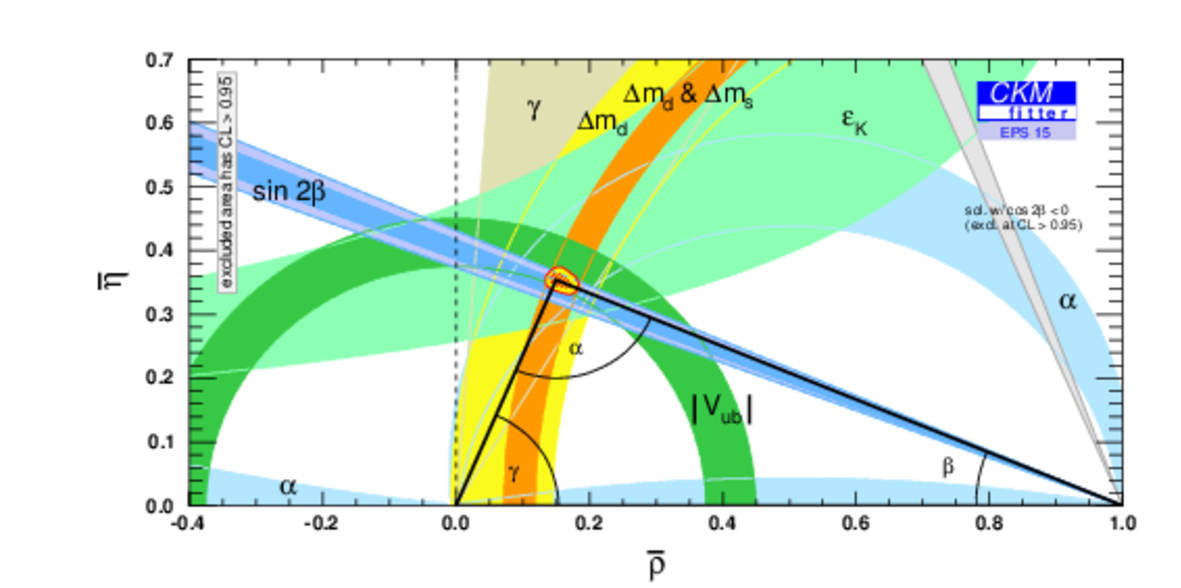
\includegraphics[width=7.5cm]{rhoeta_small_global.pdf}
\end{center}
\caption{Left plot: 68\% CL regions in $B^{0}_{s}$ width difference $\Delta\Gamma_{s}$
and weak phase $\phi_{s}$ obtained from individual and combined CDF, D0,
ATLAS, CMS and LHCb likelihoods of $B^{0}_{s}\to J/\psi\phi$, $B^{0}_{s}\to
J/\psi KK$, $B^{0}_{s}\to J\psi\pi\pi$ and $B^{0}_{s}\to D_{s}^{+}D_{s}^{-}%
$.The expectation within the Standard Model is shown as the black rectangle. Right plot: the current status of the CKM unitarity triangle test from the CKMFitter collaboration. }%
\label{figphis}%
\end{figure}




%
%\section{Charmless $b$ Hadron Decays}
%\label{sec:charmless}
%
%The study of of $b$-hadron decays to hadronic final states with no charmed particles allow for a rich array of studies. A few examples are the measurements of branching fractions, CP asymmetries, weak and strong phases and the CKM angles; they probe the dynamics of weak and strong interactions. The typical branching fractions of these modes are below $10^{-5}$ and thus their analyses are feasible only with large data samples and the use of powerful tools to reject background. The LHCb experiment is an adequate experimental environment for these analyses, offering the possibility to study decays of light $B$ mesons, $B_s$ mesons and $b$ baryons.
%
%In particular, CP-violation related studies of charmless $b$-hadron decays have a number of theoretical applications and that provide a probe to new physics, along the lines described in Sec.~\ref{sec:cpv}.
%For instance, the decays \BdtoKsPiPi and \BdtoKsKK are dominated by \btoqqbars ($q = u,d,s$)
%loop transitions.
%Mixing-induced \CP asymmetries in such decays are predicted to be approximately
%equal to those in \btoccbars transitions, \eg $\Bd\to\jpsi\KS$, by the
%Cabibbo-Kobayashi-Maskawa mechanism~\cite{Cabibbo:1963yz,Kobayashi:1973fv}.
%However, the loop diagrams that dominate the charmless decays can have
%contributions from new particles in several extensions of the Standard Model,
%which could introduce additional weak phases~\cite{Buchalla:2005us,Grossman:1996ke,London:1997zk,Ciuchini:1997zp}.
%A time-dependent analysis of the three-body Dalitz plot allows measurements of
%the mixing-induced \CP-violating
%phase~\cite{Dalseno:2008wwa,Aubert:2009me,Nakahama:2010nj,Lees:2012kxa}. 
% The current experimental measurements of \btoqqbars decays~\cite{HFAG} show
%fair agreement with the results from \btoccbars decays (measuring the weak
%phase \Pbeta) for each of the scrutinised \CP eigenstates.
%There is, however, a global trend towards lower values than the weak phase
%measured from \btoccbars decays.
%The interpretation of this deviation is made complicated by QCD
%corrections, which depend on the final state~\cite{Silvestrini:2007yf} and
%are difficult to handle.
%An analogous extraction of the mixing-induced \CP-violating phase in the
%\Bs system ($\beta_s$) will, with a sufficiently large dataset, also be possible with
%the \BstoKsKPi decay, which can be compared with that from, \eg
%$\Bs\to\jpsi\phi$.
%
%An impressive harvest of results from charmless hadronic $B$ mesons decays was obtained by the $B$ factories. Several french groups participated in these studies within the BaBar experiment, and in particular, a part of the present LPNHE-LHCb group. The LHCb experiment is already playing an important role in this area of physics, with the participation of the LPC and LPNHE groups. Both have contributed to the LHCb analysis of the decay modes \BstoKshhp ($\had^{(\prime)} = \pi, K$) with $1$~fb$^{-1}$ of data, which are being pursued with $3$~fb$^{-1}$.  In particular they are performing amplitude analyses (aka Dalitz-plot analyses) of \BdtoKsPiPi and \BdtoKsKK decays. At LHCb, the first step of the charmless $b$ hadron decays physics programme is to establish the signals of yet unobserved rare modes. The only yet-unobserved \BstoKshhp mode is \BstoKsKK. The LPC group also performs analyses of $B_s \to \rho^0 \rho^0$, and $\Lambda_b^0 (\Xi_b^0) \to p \had \had^{\prime}\had^{\prime\prime}$ decays.
%
%All the analyses mentioned above provide a long-term physics programs that can profit from the LHCb upgrade. These analyses proceed in increasingly complex steps, which become more and more sensitive to new physics observables with the growing dataset, and with more observed decay modes. One of the long-term goals is to perform full flavor- and time-dependent Dalitz-plot analyses of the \BstoKshhp modes to the measure the weak phases $\beta$ and $\beta_s$. Recent theoretical and experimental activity has focused on the determination of the CKM angle \Pgamma from charmless $B$ meson decays using and refining the methods proposed in Refs.~\cite{Ciuchini:2006kv,Gronau:2006qn,Bhattacharya:2013cla}. The LPNHE group is checking the applicability of the method described in the last reference to the LHCb physics analysis. Moreover, with the upgrade of LHCb, more modes, eventually with more neutral hadrons, are being considered.

\section{Rare, radiative and semileptonic $B$ decays}

%mediated by loop and box diagrams, where yet undiscovered particles could appear. Since particles in loops are virtual, even particles with masses  higher than the energy of the collisions could intervean in the diagrams, modifying the rates and the properties of the decay respect to  the standard model predictions. This would provide an indirect sign of new physics. 
 %(Rare decays of $B$ mesons are the most natural candidates to be studied with this approach: being dominated by the loop diagrams, they are considered suppressed in the standard model, and so  they are more sensitive to variations due to new physics.  
%The same hold for CPviolation measurements: being the CP ) 

Rare decays of $B$ mesons are natural candidates to be studied within the indirect approach: being dominated by  loop and box diagrams, they are very suppressed in the Standard Model, and so the most sensitive to variations due to new physics.  
Among them, radiative B decays, with the emission of a virtual or real photon, as well as semileptonic B decays are extremely interesting, as the theory has the instruments to perform very precise predictions.  A joint work between experimentalists and theorists has allowed to identify an ensemble of observables which are
at the same time sensitive to the couplings to different possible sources of New Physics (NP) and as immune as possible to non factorizable QCD effects. 
With the abundance of data produced by the LHC collisions, for the first time some of these decays can be observed, their properties measured  and the prediction tested with better precision than ever. 

For example , the LHCb collaboration has produced a large set of results, related to the exclusive $b \to s\ell \ell $ decay modes, which  are currently dominating the field.  
In the special case of the $\cb(B_s\to \mu\mu)$, the CMS collaboration is also significantly contributing and after combining the results of the two experiments, 
it turned out that the long searched $\cb(B_s\to \mu\mu)$ is only slightly lower than, but compatible with, the value
predicted in the Standard Model (SM). The $B_d\to \mu\mu$ decay has also been seen, its branching ratio turning out to be compatible with the value predicted by the SM. 
\par
On the other hand,  after comparing the experimental values of $B\to K^\ast \mu\mu$  angular observables, as well as of $\cb(B\to K \mu\mu)$ and $\cb(B_s\to \phi \mu\mu)$, with the theoretical estimates derived in the SM, 
one finds considerable discrepancies, of the order of 3 to 3.5 standard deviations.  The LHCb results of the $B^0\to K^\ast \mu\mu$  angular analysis were also recently confirmed  by the BELLE collaboration.  
It appears, however, that the most significant discrepancies occur near the charm production threshold, a region notoriously difficult for the theoretical 
description of these decays. In fact in this region it is required an accurate estimate of the hadronic matrix element of a non-local operator corresponding to disconnected $c\bar c$-diagrams, which 
cannot be computed by means of numerical simulations of QCD on the lattice. For that reason, as of now, it is not clear whether the current discrepancies are due to the lack of theoretical 
control of the $c\bar c$ contributions, or they indicate the presence of NP couplings. If the second option is adopted, the angular observables of $B\to K^\ast \mu\mu$ and $B_s\to \phi \mu\mu$ 
decay modes provide very stringent constraints on the scenarios of NP. 

On top of the very rich set of results involving muons, LHCb has also performed an angular analysis  of the $B^0\to K^\ast e e $ decay mode in the low dilepton invariant mass region. The results found  are in agreement with SM but currently quite limited in statistics.    With more data coming, the electron channels will be more and more competitive and their measurements more precise. Among other observables, they actually  provide a  measurement of the photon polarization, as the di-electron are emitted by a virtual photon in some part of the kinematic space.  This is a complementary measurement to the one of the decays involving real photons, like $B_s \to \phi \gamma$ and $B\to K^* \gamma$.  In the SM the photon polarization  in $b \to s \gamma$ transition is  known to be left (right) for a $b$ ($\bar b$) quark, modulo effect of the order of $4\%$  du to the quark masses and the emission of soft gluons. Any deviation from this precise expectation would be a clear sign of NP.  In the next years precise measurements of the photon polarization in $b \to s \gamma$ transitions are expected to come, but some challenges need to be faced, like for example the study of the resonant $K^*$ structure, which needs a close collaboration between theorists and experimentalists. 

Another experimental result which has also provoked some interest in the flavor physics community is that $R_K = \cb(B\to K\mu\mu)/\cb(B\to Kee)_{{\rm low}-q^2}$ was found to be $2.6\sigma$ smaller than  predicted in the SM, which suggests the violation of universality of the coupling to leptons (LFUV). Such a puzzling phenomenon should be scrutinized with higher statistics and tested in other similar situations, 
such as $R_K$ at high-$q^2$'s, $R_{K^\ast}$, $R_{\Lambda^{(\ast )}}$ at both low- and high-$q^2$. This observation is adding to an already noted problem of $R_{D^{(\ast)}}=  \cb(B\to D^{\ast}\tau\nu_\tau)/\cb(B\to D^{\ast}\mu\nu_\mu)$ for which the experimental result, first measured at the $B$-factories and then confirmed at LHCb, is $(2\div 4)\sigma$ larger than predicted in the SM. There are very few phenomenologically viable theoretical scenarios of NP which can simultaneously explain that $R_K^{\rm exp}<R_K^{\rm SM}$ and that $R_{D^{(\ast )}}^{\rm exp} > R_{D^{(\ast )}}^{\rm SM}$. To further understand the origin of the LFUV one can envisage doing the angular analysis of all the mentioned decay modes, and from the ratios of angular observables check whether or not a similar size of the LFUV is indeed observed. 
Furthermore, to facilitate a comparison with theory it is more sound to compare $B_s\to D_s^{(\ast)}\ell \nu_\ell$ because the theoretical uncertainty related to the chiral extrapolation in the light valence quark on the lattice is completely avoided in this way. Moreover, the emission of soft photons can differently affect $B^- \to D^{0 (\ast)}\ell^- \bar \nu_\ell$ and $B^0 \to D^{- (\ast)}\ell^+ \nu_\ell$, the modes which are usually averaged. Such a problem is much less significant if one works with $B_s\to D_s^{(\ast)}\ell \nu_\ell$ decays. 

Most of the models pretending to describe the LFUV effects allow for the lepton flavor violation (LFV) too. For that reason it is of great interest to measure the LFV modes such as $B_s\to \mu \tau$, $B\to K^{(\ast )}\mu \tau$,  $B_s\to \phi \mu \tau$, which can now be probed thanks to the large statistics achievable at the LHC. The experimental bounds on $\cb(B_s\to \mu e)$ and $\cb(B_s\to K^{(\ast )} \mu e)$ can also be greatly improved. These results can be very useful for phenomenology of the LFV decays and for the bigger picture that could ultimately lead to a theory of flavor of quarks and leptons. 

The French community is largely active both on the experimental and theoretical side on rare, radiative and semileptonic decays.  In the need of exchanging results, it has been promoting in the past years the aforementioned PEPS-PTI projects and the related workshops, successfully followed by the community. They clearly establishing the need of a GDR as a regular framework  were the discussions and the collaboration could take place on a more regular basis. The following topics should be addresses:
\begin{itemize}
\item For the LFUV, we should elaborate a general scenario of NP, in an effective field theory approach, allowing to isolate the  observables  which are most sensitive to the couplings to the vector (scalar) and/or axial (pseudoscalar) operators. Experimenters and theorists will elaborate on the feasibility of the distribution of $B_{(s)}\to D_{(s)}^\ast  \ell \nu_\ell$ according to the polarization of the outgoing vector meson. Furthermore, a contact with other leptonic observables should be made in order to test several plausible scenarios of NP which result in LFUV. New experimental results on the ratio measurements will be provided by LHCb, but are also expected from BelleII. 
\item For the angular analyses of $b \to sll$ transitions, with the new and more accurate experimental data, it becomes mandatory to assess the hadronic uncertainties on the theory side. Lattice QCD and the QCD sum rule practitioners will try and 
evaluate the size of theoretical errors and discuss the appropriate methodology on how to account for various sources of systematic uncertainties. We should explore the  $B^0\to K^\ast \tau\tau$ channel and define new observables taking into account the direct access to the $tau$ polarization. The study of $b \to s \ell \ell$ transition in b-baryons  is quite new and the identification of interesting observables for the $\Lambda_b \to \Lambda^\ast \mu\mu$ may be interesting.  
Possible phenomenological ideas on how to relate the hadronic quantities in several decay modes will be discussed as they might be helpful in canceling a large part of hadronic uncertainties.
Ideas on how to treat the non-resonant $c\bar c$-contributions would be very welcome. The phenomenological interpretation of the experimental results will allow to shed lights on which physics beyond standard model best fits the data. 
\item The LFV direct searches will soon provide new results. It will be crucial to work on a package that could include all the possible constraints relevant to LFV at low and high energy and see what are the lessons one can learn about the Yukawa sector from the data. 
\item Finally we should assess the current situation concerning the extraction of the Yukawa couplings from experimental data, clarifying in which way those data can be related to the low-energy physics observables and 
$b$-decay observables in particular. In order to address the issue of ``{\it Which theory of flavor?}" we will try and combine the searches made at Belle~II with those made at NA62 and KOTO experiments.  
Address the issue of (in)compatibility of the conclusions found in the Yukawa sector through the low-energy experiments with the LHC findings at the TeV-scale. 
\end{itemize} 

%%A proposed timeline for the annual workshops is described below. 
%\begin{enumerate}
%\item Year One: Workshop on the LFUV in $B$ and $B_s$ decays\\ 
%During this workshop the theorists will discuss a general scenario of NP, in an effective field theory approach, and isolate the observables which are most sensitive 
%to the couplings to the vector (scalar) and/or axial (pseudoscalar) operators. Experimenters and theorists will elaborate on the feasibility of the distribution of $B_{(s)}\to D_{(s)}^\ast  \ell \nu_\ell$ 
%according to the polarization of the outgoing vector meson. Furthermore, a contact with other leptonic observables should be made in order to test several plausible scenarios of NP which 
%result in LFUV.
%
%\vskip .6cm 
%
%\item Year Two: Workshop on the angular distribution of various decay modes\\ 
%With the new and more accurate experimental data it becomes mandatory to assess the hadronic uncertainties on the theory side. Lattice QCD and the QCD sum rule practitioners will try and 
%evaluate the size of theoretical errors and discuss the appropriate methodology on how to account for various sources of systematic uncertainties. 
%Another interesting subject could be the angular analysis of $B^0\to K^\ast \tau\tau$ and the study of new observables taking into account the direct access to the $tau$ polarization.
%The study of $b \to s \ell \ell$ transition in b-baryons  is quite new and the identification of interesting observables for the $\Lambda_b \to \Lambda^\ast \mu\mu$ may be interesting.  
%Possible phenomenological ideas on how to relate the hadronic quantities in several decay modes will be discussed as they might be helpful in cancelling a large part of hadronic uncertainties.
%Ideas on how to treat the non-resonant $c\bar c$-contributions would be very welcome. Participants will also address the question {\it ``Which physics BSM?"}
%
%\vskip .6cm 
%
%\item Year Three: Workshop on the lepton flavor violation in $b$-decays\\ 
%Revisiting the LFUV problem: discuss the new constraints on  $R_{K^{(\ast )}, D^{(\ast )}, \Lambda^{(\ast )}}$ obtained in Belle~II, and attempt drawing more accurate conclusions concerning the 
%new physics scenarios. Focus then on the LFV modes and on interpretation of the results found by LHCb. The issues related to the identification of $\tau$ in the final state should be revisited. 
%Work on the package of codes that would include all possible constraints relevant to the LFV at low and high energy and see what are the lessons one can learn about the Yukawa sector from the data. 
%
%\vskip .6cm 
%
%\item Year Four: Workshop on the relation to Higgs \\ 
%Assess the current situation concerning the extraction of the Yukawa couplings from experimental data. In what way those data can be related to the low-energy physics observables and 
%$b$-decay observables in particular. In order to address the issue of ``{\it Which theory of flavor?}" we will try and combine the searches made at Belle~II with those made at NA62 and KOTO experiments. 
%Address the issue of (in)compatibility of the conclusions found in the Yukawa sector through the low-energy experiments with the LHC findings at the TeV-scale. 
%
%\end{enumerate}


\section{Charm and Kaon Physics}

In the LHC collisions, a large part of the proton-proton cross section goes into charm and strange quarks production.  Indeed, the $c \bar{c}$ cross-section is roughly 10\% of the total inelastic cross-section, so that charm hadrons are produced extremely copiously. Their short but measurable decay times make them relatively simple to reconstruct and separate from background.The LHCb detector has developed dedicated triggers registering  large samples of charm hadron decays and is currently exploring the best strategy to collect a large quantity of kaon decays. In fact, charm and kaon physics provides complementary insights into flavor physics to this obtained from the $b$ sector. 

Precise studies of the properties and decays of charmed hadrons are motivated as almost-null tests of the Standard Model. In terms of CP violation, charm hadron decays involve only the first two generations of quarks, and the CP violation in decay is therefore expected to occur at below the per mil level in the SM. Additionally, compared to beauty or strange hadrons, the mixing of neutral charm hadrons is slow, with both the $x = \Delta m/\Gamma$ and $y = \Delta \Gamma/ (2\Gamma)$ parameters at around the percent level. The CP violation in charm decays has not been observed so far, and the existing experimental limits are at the few per mil level. The theoretical predictions of charm CPV are difficult as long distance contributions dominate; CPV in decay close to the present experimental limits could be accommodated within the SM or could be signs of NP, and a progress on the theory side is required to disentangle the two. Similarly, in the case of mixing, or CP violation in the interference of decay and mixing, more precise experimental results are needed to stimulate progress on the theoretical predictions.

In addition, charmed hadrons are also an interesting place to study rare and forbidden transitions, for example FCNS or lepton number violating decays. The most recent studies of charmed hadron decays within the French community were performed on the rare decays $D^0 \to \pi \mu\mu$ (with same sign muons) and $D^0 \to K \pi\mu\mu$. The former is of interest because the copious production rate of charmed hadrons allows effective limits to be placed on Majorana neutrinos. The latter is the charmed counterpart of $B\to K^*\mu\mu$ and has now been observed for the first time by LHCb, albeit within a dimuon $q^2$ region dominated by the $\omega$ and $\rho$ resonances. It should in principle share much of the same phenomenology of $B\to K^*\mu\mu$,  with the complication of much higher backgrounds from decays to hadronic resonances (such as $K\pi\rho$) which subsequently decay to dimuon pairs. Once that a large signal yields become available, an angular analysis will be of prior interest. 

In the upcoming period, the most critical work will be to improve the limits on CPV, both in decay and the interference of mixing and decay, as well as to make ever more precise measurements of charm mixing parameters using both the $D\to hh$ and $D\to K_s hh$ decay modes with the full Run II LHCb dataset. In addition, LHCb should obtain large samples of FCNC decays such as $D^0\to K \pi\mu\mu$, potentially allowing for an observation of the nonresonant (in the dimuon spectrum) decay and a measurement of angular observables similar to the ones which characterise $B\to K^*\mu\mu$. Finally, making more precise measurements of charm hadron lifetimes, in particular in the less well understood baryon sector, could aid the development of HQE tools and techniques required to eventually obtain precise SM predictions for mixing and CPV in the charm sector.


Concerning kaon physics, it is worth to remember that kaon mixing and decays belong traditionally to the most constraining processes for physics beyond the SM. Nowadays, the discrepancies found in recent LHCb and $B$-factory data, in particular in the quantity known as $R_K$ \cite{Aaij:2014ora},  provide motivations for searches of certain $K$ decays, in particular lepton-flavor violating (LFV) ones of the kind $K \to (\pi) e \mu$.  Interestingly, the $R_K$ effect is consistent in magnitude and size with other discrepancies observed in the flavor sector. Without further assumptions, LFNU at a non-SM level implies LFV at a non-SM level. In fact, to account for $R_K$ one needs to invoke new interactions distinguishing between leptons of different generations, for example lepton-lepton couplings with a new vector boson or quark-lepton couplings with a scalar leptoquark. The fermions involved in such interactions are generally not in the mass eigenbasis -- this basis doesn't even exist at the scale of these interactions, usually above the EWSB scale. After EWSB, rotation of the quark and lepton fields to the mass eigenbasis generates LFV effects along with the LFNU ones.

One theoretically appealing way to generate new-physics shifts of the required size is to invoke an effective interaction involving dominantly quarks and leptons of the third generation \cite{Glashow:2014iga}. Then, the amount of LNU pointed to by $R_K$ actually allows to quantify rather generally the expected amount of LFV to be in the ballpark of $10^{-8}$, which happens to be within reach at LHCb's run 2. This argument, reported in Refs. \cite{Guadagnoli:2016erb,Glashow:2014iga}, motivates searches of LFV $B$ decays as a promising direction at LHCb.

This very argument has implications in $K$ physics as well, in decays of the kind $K \to (\pi) \ell \ell'$, such as $K_L \to e^\pm \mu^\mp$ and $K^+ \to \pi^+ e^\pm \mu^\mp$. Experimental limits on these modes are more than ten years old: $\mc B(K_L \to e^\pm \mu^\mp) < 4.7 \times 10^{-12}$ \cite{Ambrose:1998us}, $\mc B(K^+ \to \pi^+ e^- \mu^+) < 1.3 \times 10^{-11}$ \cite{Sher:2005sp}, $\mc B(K^+ \to \pi^+ e^+ \mu^-) < 5.2 \times 10^{-10}$ \cite{Appel:2000tc}. Theoretical expectations for the above decays are straightforwardly calculable after suitably normalising the decay modes of interest in order to cancel phase-space factors. Defining $\beta^{(K)}$ as the ratio of the new-physics Wilson coefficient responsible for the decay in the numerator over the SM Wilson coefficient responsible for the normalising decay, we get
\bea
\label{eq:LFV_K_decays}
\frac{\Gamma(K_L \to e^\pm \mu^\mp)}{\Gamma(K^+ \to \mu^+ \nu_\mu)} = | \beta^{(K)} |^2~, \\
\label{eq:LFV_K_decays_2}
\frac{\Gamma(K^+ \to \pi^+ \mu^\pm e^\mp)}{\Gamma(K^+ \to \pi^0 \mu^+ \nu_\mu)} = 4 | \beta^{(K)} |^2~.
\eea

To get a numerical idea of the effects to be expected, we need a model predicting $|\beta^{(K)}|^2$. For the sake of definiteness, here we use ``model A'' of Ref. \cite{Guadagnoli:2015nra} (any other motivated model, for example Ref. \cite{Boucenna:2015raa}, will do), thereby obtaining $| \beta^{(K)} |^2 = 2.15 \times 10^{-14}$. Use of eqs. (\ref{eq:LFV_K_decays}) then implies
\be
\label{eq:KLemu}
\mc B(K_L \to e^\pm \mu^\mp) \approx 6 \times 10^{-14}~,
\ee
where we have used $\mc B(K^+ \to \mu^+ \nu_\mu) \approx 64\%$ and $\Gamma(K^+) / \Gamma(K_L) \approx 4.2$ \cite{Agashe:2014kda}. In addition
\be
\mc B(K^+ \to \pi^+ e^\pm \mu^\mp) \approx 3 \times 10^{-15}~.
\ee
after use of $\mc B(K^+ \to \pi^0 \mu^+ \nu_\mu) \approx 3\%$.

While the $K^+$ LFV mode is clearly too suppressed (within the considered model!), the $K_L$ one, eq. (\ref{eq:KLemu}), has a branching ratio close to $10^{-13}$. Such a rate may actually well be reachable at the NA62 experiment. As concerns LHCb, it should be noted that, although $K$ mesons are produced copiously, their lifetimes are typically too long for the detector size -- with the exception of the $K_S$. A dedicated study is thus necessary to understand the actual LHCb capabilities for the above decays.


\bibliographystyle{JHEP}
\bibliography{charm_and_K}

%\end{document}


\include{LeptonFlavor}

\include{HFprodAndSpectro}


\section{Future Experiments}

There are a large variety of future experiments at the intensity frontier planned in the coming years. Here we have divided them into two categories: those searching directly for physics beyond the Standard Model, and flavour physics experiments which can indirectly probe high energy scales through precision measurements. 

\subsection{Weakly interacting new light particles searches}

In this subsection we focus on searches for weakly interacting new light particles, commonly called WISPs, of which the two canonical candidates are hidden photons and axion-like particles. Experiments to search for these are in many cases very cheap, and can often recycle older experiments. 


The best motivated WISP is the QCD axion itself, which is expected to solve the strong CP problem but is associated with new physics above $10^9$ GeV. Its mass may lie anywhere in the sub-eV range, and it is a very well-motivated dark matter candidate. 


Axion-like particles (ALPs) are (pseudo)-scalars, perhaps cousins of the QCD axion but which do not obtain their masses from QCD. They are characterised by their coupling to photons in a Lagrangian term $\mathcal{L} \supset - \frac{1}{4} g_{a\gamma \gamma} a F_{\mu \nu} \tilde{F}^{\mu \nu}.$ These are highly motivated from top-down constructions as generically arising when symmetries are broken at high scales, and also make attractive dark matter candidates. On the other hand, and perhaps most importantly, there have recently been several studies indicating possible discoveries of such particles in various astronomical observations: either as an explanation for excessive white dwarf cooling or anomalous transparency of the universe to gamma rays, and most excitingly as an explanation for the soft excess of X-rays from the coma cluster (at $200$ eV) and/or the oscillatory modulation of X-rays from the Perseus cluster (and even, perhaps, an explanation for an observed $3.55$ keV X-ray line). These hints all point to a very light ALP ($< 10^{-12}$ eV) with a coupling $g_{a\gamma \gamma} \sim \mathcal{O}(10^{-11} \div 10^{-12}) \mathrm{GeV}^{-1}.$ However, while this is a very interesting region to probe, such a particle could have a wide range of masses and couplings. 



Hidden photons are new (massive) gauge bosons which mix kinetically with the visible photon via a dimensionless kinetic-mixing parameter $\chi$. While one motivation of these is as a possible explanation for the $3\sigma$ discrepancy between the measured and calculated value of the muon dipole moment -- this would require a hidden photon in the $\mathcal{O}(100)$ MeV range with $\chi \sim \mathcal{O}(10^{-3})$ -- they also appear generically in top-down constructions of beyond-the-Standard Model physics. They have been proposed as perhaps the most natural force carriers for light dark matter particles, or could even make up the dark matter themselves. Intensity frontier experiments searching for these either search for the particles as dark matter or attempt to directly produce them. In the dark matter case, the assumption that there is a large abundance of particles all around us greatly enhances the reach; on the other hand, for the very light ALPs this is unlikely to be the case. The dark matter searches consist of resonant cavities, helioscopes, and now many more exotic suggestions. Direct searches are broadly photon regeneration experiments (light shining through a wall), electron colliders or beam dumps. 

Important upcoming experiments include:
\begin{itemize}
\item Axion haloscopes (magnetic resonant cavity experiments) ADMX-HF, YMCE and WISPDMX at the University of Washington, Yale and Hamburg respectively are all expected to report results soon, probing axion masses in the $\mu$eV range. 
\item The FUNK experiment in Karlsruhe uses a dish antenna to search for dark matter hidden photons.
\item The helioscope SHIPS at Hamburg searches for hidden photons produced in the sun.
\item The REAPR and ALPS-II photon regeneration experiments at Fermilab and DESY respectively will attempt to directly produce ALPs or hidden photons in the lab.
\item The IAXO helioscope at CERN uses a magnetic field to search for ALPs produced in the sun. It is expected to operate over the next decade and there are significant synergies with the French community.
\item The SHIP  beam dump experiment using the SPS proton beam at CERN has a substantial input from French theorists and experimentalists. It has the potential to search for particles in the GeV range, which included heavier ALPs, as well as other candidates such as right-handed neutrinos. Its development will encompass much of the lifetime of the proposed GDR.
\item There will be electron beam-dump experiments HPS, DarkLight and MESA at SLAC, JLab and Mainz respectively, with the latter running in about 2020. These will provide high intensity competition to hidden-photon searches in the $10-1000$ MeV range.
\item The BMV experiment at Toulouse received ANR funding in 2014 to build phase two and complement its 2007 results. It can perform photon regeneration searches; it also included an X-ray regeneration experiment.
\item There is also a proposal to use the Tore Supra tokamak at Cadarache to search for ALPs. This would be particularly interesting to unite with the plasma physics community. 
\end{itemize}





\subsection{Future experimental programs related to $CP$ violation, rare decays of heavy flavours and lepton flavour violating processes}   

As far as $CP$ violation and rare $b$-flavoured hadrons or $\tau$ decays are concerned, the two main players at the horizon of 2025 are the  upgraded LHCb experiment at CERN and the Belle II experiment at KEK.  The synergie and complementarity between the two projects has been assessed clearly in the past and we should ensure within the GDR to follow the progress in both the collaborations. In this respect, we can profit of the connexions established already by members of the GDR with the KEK collegues in the framework of the TYL/FJPPL (Franco-Japan Particle Physics Laboratory) . 

Several large or medium scale projects related to Flavour Physics are envisaged to probe Beyond Standard Model Physics. Among them, there are prospective studies to educate the possibility to run the LHCb spectrometer in the High Luminosity phase of the LHC or to make use of high intensity beam lines ({\it e.g.} SPS and FCC injectors)  with fixed target experiments.            

A possible long-term strategy for high-energy physics at colliders, after the exploitation of the LHC and its High Luminosity upgrade, considers a tunnel of about 100 km circumference, which takes advantage of the present CERN accelerator complex. The Future Circular Collider (FCC) concept follows on the successful experience and outcomes of the LEP-LHC complex of experiments. A possible first step of the project is to fit in the tunnel a high-luminosity $e^+e^-$ collider aimed at studying comprehensively the electroweak scale with centre-of-mass energies ranging from the $Z$ pole up to beyond the $t \bar t$ production threshold. A  100 TeV proton proton collider is considered as the ultimate goal of the project.  
Future Circular Collider study groups have been formed in a design study hosted by CERN, aiming at a Conceptual Design Report and a review cost in time for next European Strategy milestone (2018-2019). The unprecedented statistics at the $Z$ pole (${\cal O}(10^{12-13} Z$ decays) potentially delivered by the high-luminosity $e^+e^-$ collider can be studied in particular to explore further the Flavour Physics case at large.  

In that framework, several French teams, gathering small groups of experimentalists and phenomenologists, are contributing to the design study in Flavour studies.  
There is a Physics potential of the measurements of rare decays of $b$-hadrons, which can complement  the anticipated results from the current and foreseen $b$-Physics programs (LHCb upgrade and SuperKEKB $B$-factory). In that respect, French contributions are mainly focused on rare electroweak penguins which are likely unique to the FCC: $B^0 \to K^*(892) \tau^+\tau^-$ and $B_s \to \tau^+ \tau^-$.   
The large statistics at the $Z$ pole can be used as well to scrutinize in particular Lepton Flavour Violating (LFV) $Z$ decays, which would serve as an indisputable evidence for New Physics if seen. Heavy right-handed neutrals are natural candidates to explain LFV phenomena. They can be as well searched for directly at FCC-$ee$. A number of low energy experiment are addressing this very question through the search for LFV by muon capture on nuclei ({\it e.g.} COMET in Japan) or the radiative decay of large ensemble of muons ({\it e.g.} MEG in Europe). 

One objective of the GDR is to address the complementarity of these high intensity machines,  at large scale apparatus or low-energy experiments.       



\section{Conclusion}
The intensity frontier is a strategic approach to search for new physics.  Its validity is recognized at an international level and  it is a domain in which the French particle physics community is traditionally very active. Interesting and puzzling results are being produced by the experiments currently taking data, and further more are expected to come from the new generation of experiments that are starting or being planned. Theoretical progress are ensuring the precision of the currently performed tests, and additional clean observables are under investigation. 

The French community working in this field recognizes the need of coming together to pursue these searches together with a renewed enthusiasm  and with a stronger collaboration between the experimental and the theoretical laboratories in France.   
The GDR intensity frontier will be the place where we will be able to put together our experience, share our knowledge, renforce bounds and inspire new collaborations, ensuring that the French community continues to be competitive and focused on the most appealing topics of the field. It will additionally provide a forum to discuss the future of the field, and naturally promote the emergence of a young and dynamic generation of physicists. All this will allow to keep the current involvement and acquire an even higher visibility at a national and international level.




%----------------------------------------------------------------------------------------
%	BIBLIOGRAPHY
%----------------------------------------------------------------------------------------

\bibliographystyle{apalike}

\bibliography{sample}

%----------------------------------------------------------------------------------------


\end{document}